\section{Vector-Valued Functions} \label{S:9.6.Vector_Valued_Functions}

\vspace*{-14 pt}
\framebox{\hspace*{3 pt}
\parbox{6.25 in}{\begin{goals}
  \item What is a vector-valued function? What do we mean by the graph
    of a vector-valued function?
  \item What is a parameterization of a curve in $\R^2$? In $\R^3$?
    What can the parameterization of a curve can tell us?
\end{goals}} \hspace*{3 pt}}

\subsection*{Introduction}

So far, we have seen several different examples of curves in space,
including traces and contours of functions of two variables, as well
as lines in 3-space.  Recall that for a line through a fixed point
$\vr_0$ in the direction of vector $\vv$, we may express the line
parametrically through the single vector equation
$$\vr(t) = \vr_0 + t\vv.$$
From this perspective, the vector $\vr(t)$ is a function that depends
on the parameter $t$, and the terminal points of this vector trace out
the line in space.

Like lines, other curves in space are one-dimensional objects, and
thus we aspire to similarly express the coordinates of points on a
given curve in terms of a single variable.  Vectors are a perfect
vehicle for doing so -- we can use vectors based at the origin to
identify points in space, and connect the terminal points of these
vectors to draw a curve in space.  This approach will allow us to draw
an incredible variety of graphs in 2- and 3-space, as well as to
identify and describe curves in $n$-space for any $n$.

\begin{pa} \label{PA:9.6} In this activity we consider how we might use vectors to define a curve in space.
    \ba
    \item On a single set of axes in $\R^2$, draw the vectors $\left\langle \cos(0), \sin(0) \right\rangle$, $\left\langle \cos\left(\frac{\pi}{2}\right), \sin\left(\frac{\pi}{2}\right) \right\rangle$, 
    
     $\left\langle \cos\left(\pi\right), \sin\left(\pi\right) \right\rangle$,  \text{ and } $\left\langle \cos\left(\frac{3\pi}{2}\right), \sin\left(\frac{3\pi}{2}\right) \right\rangle$ with their initial points at the origin.


    \item On the same set of axes, draw the vectors $\left\langle \cos\left(\frac{\pi}{4}\right), \sin\left(\frac{\pi}{4}\right) \right\rangle$, $\left\langle \cos\left(\frac{3\pi}{4}\right), \sin\left(\frac{3\pi}{4}\right) \right\rangle$, 
    
     $\left\langle \cos\left(\frac{5\pi}{4}\right), \sin\left(\frac{5\pi}{4}\right) \right\rangle$,  \text{ and } $\left\langle \cos\left(\frac{7\pi}{4}\right), \sin\left(\frac{7\pi}{4}\right) \right\rangle$ with their initial points at the origin.



   \item Based on the pictures from parts (a) and (b), sketch the set
     of \emph{terminal} points of all of the vectors of the form
     $\langle \cos(t), \sin(t) \rangle$, where $t$ assumes values from
     0 to $2 \pi$. What is the resulting figure? Why?


    \ea

\end{pa} 

\begin{activitySolution}
    \ba
    \item The vectors are shown at left in the figure below. 
  %  \begin{figure}[ht]
      \begin{center}
      \resizebox{!}{2.5in}{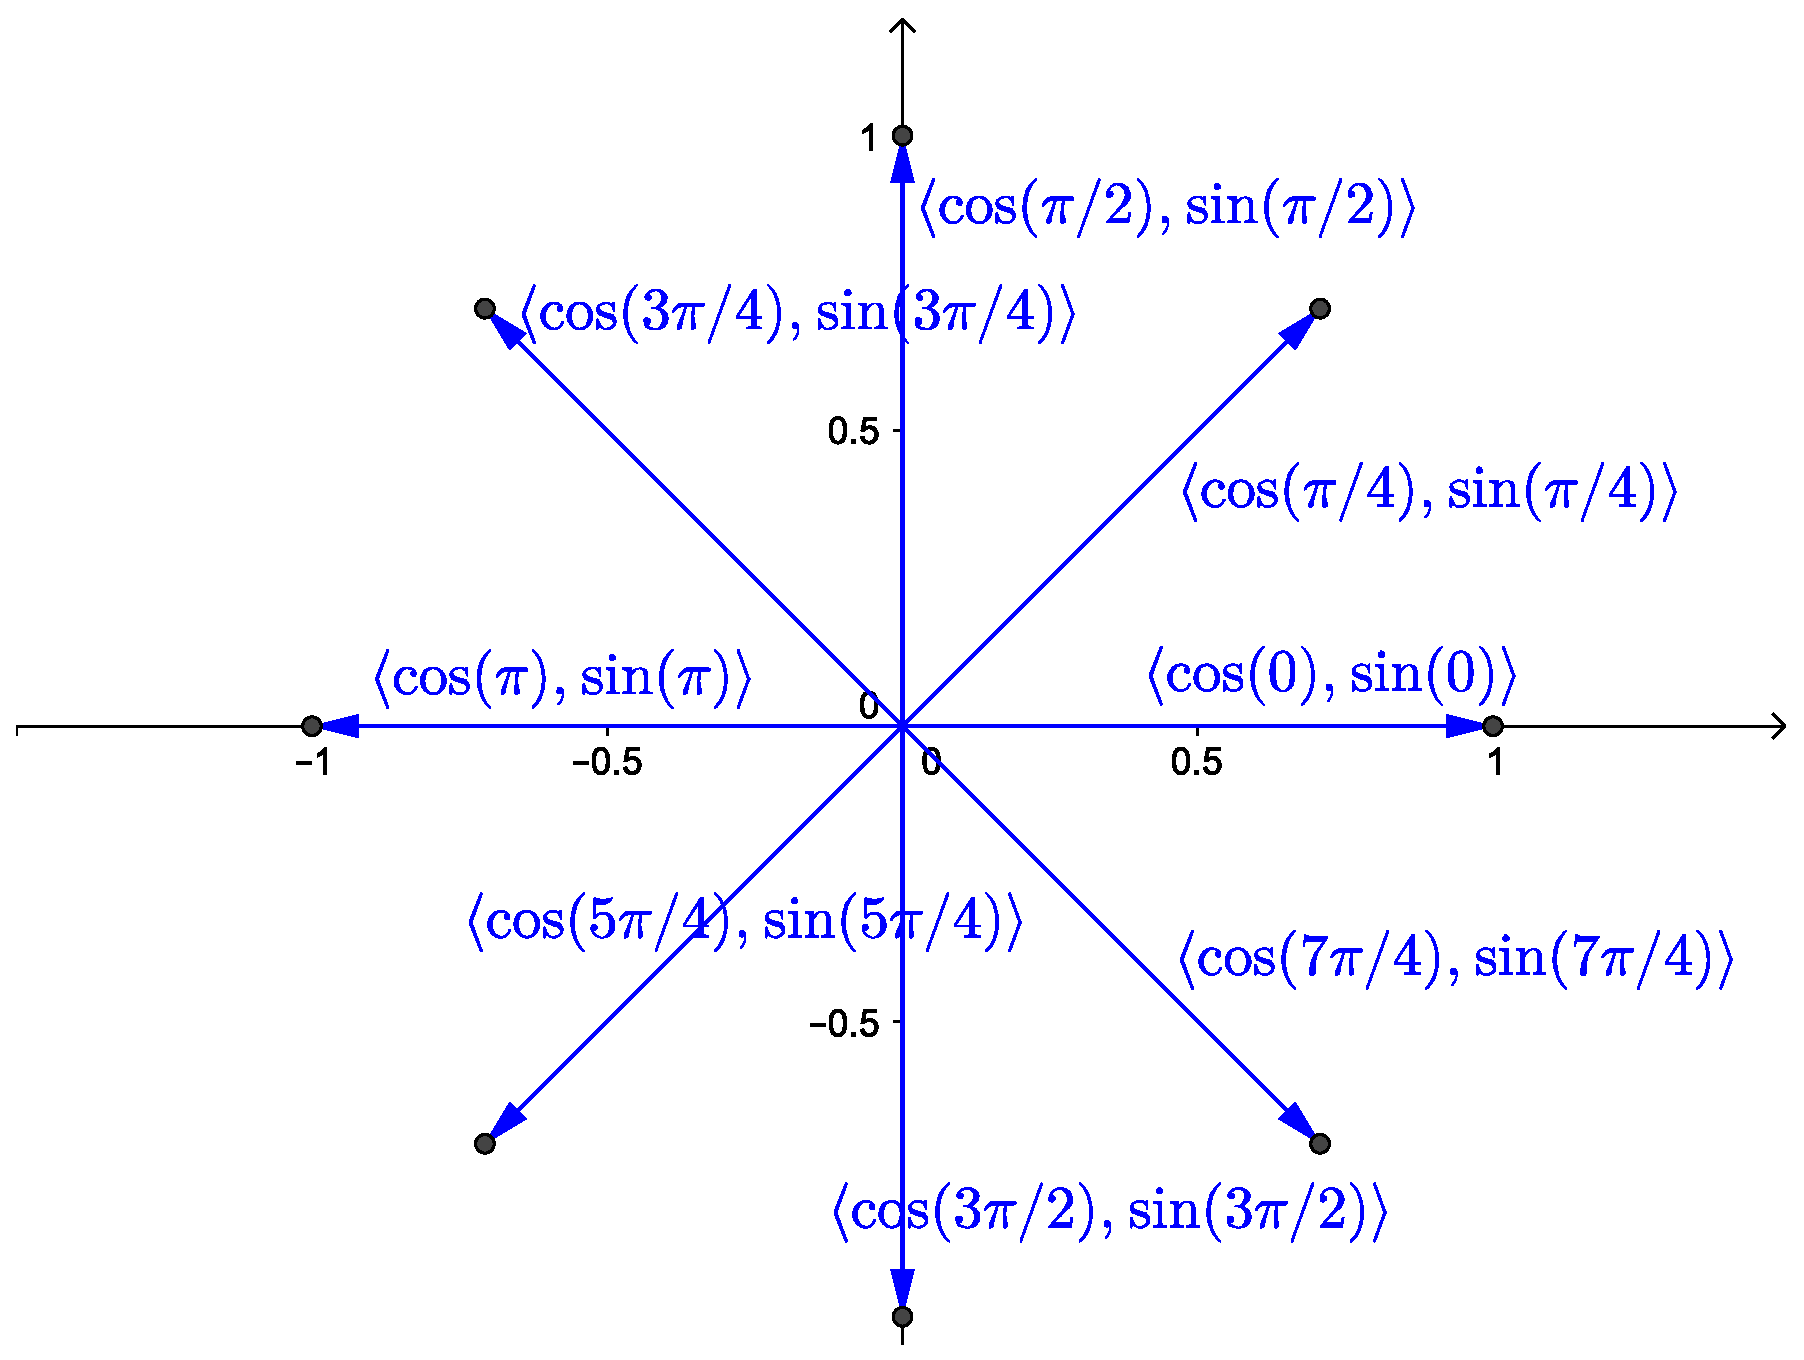
\includegraphics{figures/fig_9_6_PA_a.eps}} \resizebox{!}{2.5in}{\includegraphics{figures/fig_9_6_PA_b.eps}}
  %       \caption{For part (f)}
 %       \label{F:9.3.preview.3}
      \end{center}
  %  \end{figure}
    

    \item The vectors are shown at left in the figure above. 


   \item The terminal points of these vectors all have the form $(\cos(t), \sin(t))$. Since $\cos^2(t) + \sin^2(t) = 1$, these points all lie on the unit circle as illustrated at right in the figure above.


    \ea
\end{activitySolution}

\afterpa 

\subsection*{Vector-Valued Functions}

Consider the curve shown in Figure \ref{F:9.6.VVF_graph}. As in
Preview Activity \ref{PA:9.6}, we can think of a point on this curve
as resulting from a vector from the origin to the point. As the point
travels along the curve, the vector changes in order to terminate at
the desired point. %An animation is provided in Figure \ref{F:9.6.VVF_animation}.
A few still pictures of this motion are shown in Figure \ref{F:9.6.VVF_graph}.

\begin{figure}[ht]
\begin{center}
%\begin{minipage}{2.5in}
%\begin{center}
%\resizebox{!}{1.25in}{\includegraphics{9_6_VVF_graph1}}
%  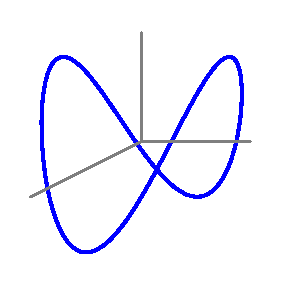
\includegraphics{figures/fig_9_6_curve_1.eps}
\resizebox{!}{1.5in}{\includegraphics{figures/fig_9_6_curve_animate_01.pdf}} \hspace{0.25in} \resizebox{!}{1.5in}{\includegraphics{figures/fig_9_6_curve_animate_25.pdf}} \hspace{0.25in} \resizebox{!}{1.5in}{\includegraphics{figures/fig_9_6_curve_animate_40.pdf}}
%\end{center}
%\ \vspace{0.075in} \
\caption{The graph of a curve in space.}
\label{F:9.6.VVF_graph}
%\end{minipage} \hspace{0.15in}
%\begin{minipage}{2.5in}
%\begin{center}
%\resizebox{!}{2.5in}{\animategraphics[controls]{4}{9_6_VVF_}{00}{20}}
%\animategraphics[controls]{4}{figures/fig_9_6_curve_animate_}{00}{50}
%\end{center}
%\caption{The vector-valued function.}
%\label{F:9.6.VVF_animation}
%\end{minipage}
\end{center}
\end{figure}



Thus, we can think of the curve as a collection of terminal points of
vectors emanating from the origin. We therefore view a point traveling
along this curve as a function of time $t$, and define a function
$\vr$ whose input is the variable $t$ and whose output is the vector
from the origin to the point on the curve at time $t$.  In so doing,
we have introduced a new type of function, one whose input is a scalar
and whose output is a vector.

The terminal points of the vector outputs of $\vr$ then trace out the
curve in space. From this perspective, the $x$, $y$, and $z$
coordinates of the point are functions of time, $t$, say
\[x = x(t), \ \ \ y = y(t), \ \ \ \text{ and } \ \ \ \ \ z = z(t), \]
and thus we have three coordinate functions that enable us to
represent the curve. The variable $t$ is called a \emph{parameter} and
the equations $x = x(t)$, $y = y(t)$, and $z = z(t)$ are called
\emph{parametric equations} (or a \emph{parameterization of the
  curve}). The function $\vr$ whose output is the vector from the
origin to a point on the curve is defined by
\[\vr(t) = \langle x(t), y(t), z(t) \rangle.\]
Note that the input of $\vr$ is the real-valued parameter $t$ and the
corresponding output is vector $\langle x(t), y(t), z(t)
\rangle$. Such a function is called a \emph{vector-valued function}
because each real number input generates a vector output.  More
formally, we state the following definition.

\vspace*{5pt}
\nin \framebox{\hspace*{3 pt}
  \parbox{6.25 in}{\begin{definition} A \textbf{vector-valued
        function}\index{vector-valued function!definition} is a
      function whose input is a real parameter $t$ and whose output is
      a vector that depends on $t$. The {\bf graph}\index{graph of a
        vector-valued function!definition} of a vector-valued function
      is the set of all terminal points of the output vectors with
      their initial points at the origin. \end{definition}

    {\bf Parametric equations}\index{parametric equations for a
      curve}\index{parameterization!curve} for a curve are equations
    of the form
\[x = x(t), \ \ \ y = y(t), \ \ \ \text{ and } \ \ \ \ \ z = z(t)\]
that describe the $(x,y,z)$ coordinates of a point on a curve in $\R^3$. \\
} \hspace*{3 pt}}
\vspace*{5pt}

Note particularly that every set of parametric equations determines a
vector-valued function of the form
\[\vr(t) = \langle x(t), y(t), z(t) \rangle,\]
and every vector-valued function defines a set of parametric equations
for a curve.  Moreover, we can consider vector-valued functions and
parameterizations in $\R^2$, $\R^4$, or indeed a real space of any
dimension.  As a reminder, in Section~\ref{S:9.5.Lines_Planes}, we
determined the parametric equations of a line in space using a point
and a direction vector.  For a nonlinear example, the curve in Figure
\ref{F:9.6.VVF_graph} has the parametric equations
\[x(t) = \cos(t), \ \ \ y(t) = \sin(t), \ \ \ \text{ and } \ \ \ z(t)
= \cos(t) \sin(t).\] Represented as a vector-valued function $\vr$,
the curve in Figure \ref{F:9.6.VVF_graph} is the graph of
\[\vr(t) = \langle \cos(t), \sin(t), \cos(t) \sin(t) \rangle.\]

%WolframAlpha notation ParametricPlot3D[{2t, Cos[t]^2, t}, {t, 0, 10}]
%3D only \url{http://cs.jsu.edu/mcis/faculty/leathrum/Mathlets/parapath.html}
%\url{http://dlippman.imathas.com/g1/GrapherLaunch.html}

\begin{activity} \label{A:9.6.1} The same curve can be represented
  with different parameterizations. Use your calculator,\footnote{If
    you have a graphing calculator you can draw graphs of
    vector-valued functions in $\R^2$ using the parametric mode (often
    found in the MODE menu).} Wolfram$\mid$Alpha, or some other
  graphing device\footnote{e.g.,
    \url{http://webspace.ship.edu/msrenault/ggb/parametric_grapher.html}}
  to plot the curves generated by the following vector-valued functions. Compare and contrast the graphs -- explain
  how they are alike and how they are different.  \ba
    \item $\vr(t) = \langle \sin(t), \cos(t) \rangle$



    \item $\vr(t) = \langle \sin(2t), \cos(2t) \rangle$



    \item $\vr(t) = \langle \cos(t+\pi), \sin(t+\pi) \rangle$



    \ea

\end{activity}
\begin{smallhint}

\end{smallhint}
\begin{bighint}

\end{bighint}
\begin{activitySolution}
    \ba
    \item The graph of $\vr(t) = \langle \sin(t), \cos(t) \rangle$ is the unit circle. The fact that $\vr(0) = \langle 0,1 \rangle$ and $\vr\left(\frac{\pi}{2}\right) = \langle 1,0 \rangle$ indicates that this parameterization traces out the unit circle in a clockwise manner.  The parameterization also traces out each quadrant using the same length interval, e.g., the graph is in the first quadrant when $t$ is between 0 and $\frac{\pi}{2}$, and in the fourth quadrant for $t$ between $\frac{\pi}{2}$ and $\pi$), which illustrates that the parameterization traces out the circle in a uniform manner.
    \item The graph of $\vr(t) = \langle \sin(2t), \cos(2t) \rangle$ is again the unit circle. In this case, we have $\vr(0) = \langle 0,1 \rangle$ and $\vr\left(\frac{\pi}{4}\right) = \langle 1,0 \rangle$, which indicates that this parameterization traces out the unit circle in a clockwise manner.  The parameterization also traces out each quadrant using the same length interval, e.g., the graph is in the first quadrant when $t$ is between 0 and $\frac{\pi}{4}$, and in the fourth quadrant for $t$ between $\frac{\pi}{4}$ and $\frac{\pi}{2}$) illustrates that the parameterization traces out the circle in a uniform manner. However, the $t$ intervals in which this parameterization lies in a given quadrant are half as long as those in part (a), which tells us that this parameterization traces out the unit circle in half the time, or twice as fast as the parameterization in part (a). 
    \item The graph of $\vr(t) = \langle \cos(t+\pi), \sin(t+\pi) \rangle$ is again the unit circle. In this case, we have $\vr(0) = \langle -1,0 \rangle$ and $\vr\left(\frac{\pi}{2}\right) = \langle 0,-1 \rangle$, which indicates that this parameterization traces out the unit circle in a counterclockwise manner.  The parameterization also traces out each quadrant using the same length interval, e.g., the graph is in the third quadrant when $t$ is between 0 and $\frac{\pi}{2}$, and in the fourth quadrant for $t$ between $\frac{\pi}{4}$ and $\frac{\pi}{2}$), which illustrates that the parameterization traces out the circle in a uniform manner and at the same rate as the parameterization in part (a) (but in the opposite direction). 
    \ea
\end{activitySolution}
\aftera


The examples in Activity \ref{A:9.6.1} illustrate that a
parameterization allows us to look not only at the graph, but at the
direction and speed at which the graph is traversed as $t$ changes. In
the different parameterizations of the circle, we see that we can 
start at different points and move around the circle in either
direction.  The calculus of vector-valued functions -- which we will
begin to investigate in
Section~\ref{S:9.7.Vector_Valued_Functions_Derivatives} -- will enable
us to precisely quantify the direction, speed, and acceleration of a
particle moving along a curve in space.  As such, describing curves
parametrically will allow us to not only indicate the curve itself,
but also to describe how motion occurs along the curve.

%\begin{activity} \label{A:9.6.2} Find a vector-valued function $\vr$ that describes a point traveling along the unit circle so that at time $t=0$ the point is at $\left(\frac{\sqrt{2}}{2}, \frac{\sqrt{2}}{2} \right)$ and travels clockwise along the circle as $t$ increases.

\end{activity}
\begin{smallhint}

\end{smallhint}
\begin{bighint}

\end{bighint}
\begin{activitySolution}

\end{activitySolution}
\aftera




Using parametric equations to define vector-valued functions in two
dimensions is much more versatile than just defining $y$ as a function
of $x$. In fact, if $y = f(x)$ is a function of $x$, then we can
parameterize the graph of $f$ by
\[\vr(t) = \langle t, f(t) \rangle,\]
and thus every single-variable function may be described
parametrically.  In addition, as we saw in Preview Activity
\ref{PA:9.6} and Activity \ref{A:9.6.1}, we can use vector-valued
functions to represent curves in the plane that do not define $y$ as a
function of $x$ (or $x$ as a function of $y$).\footnote{As an aside,
  vector-valued functions make it easy to plot the inverse of a
  one-to-one function in two dimensions. To see how, if $y = f(x)$
  defines a one-to-one function, then we can parameterize this
  function by $\vr(t) = \langle t, f(t) \rangle$. Since the inverse
  function just reverses the role of input and output, a
  parameterization for $f^{-1}$ is $\langle f(t), t \rangle$.}

\begin{activity} \label{A:9.6.3} Vector-valued functions can be used to generate many interesting curves. Graph each of the following using an appropriate tool\footnote{e.g., the 2D grapher at \url{http://webspace.ship.edu/msrenault/ggb/parametric_grapher.html}, or for 3D graphs Wolfram$\mid$Alpha, an on-line 3D grapher like \url{http://www.math.uri.edu/~bkaskosz/flashmo/parcur/}, or some other device}, and then write one sentence for each function to describe the behavior of the resulting curve.
	\ba
	\item $\vr(t) = \langle t\cos(t), t\sin(t) \rangle$

	\item $\vr(t) = \langle \sin(t)\cos(t), t\sin(t) \rangle$

	\item $\vr(t) = \langle t^2\sin(t)\cos(t), 0.9t\cos(t^2), \sin(t) \rangle$
	
	\item $\vr(t) = \langle \sin(5t), \sin(4t) \rangle$

	\item Experiment with different formulas for $x(t)$ and $y(t)$ and ranges for $t$ to see what other interesting curves you can generate.  Share your best results with peers.

	\ea

\end{activity}
\begin{smallhint}

\end{smallhint}
\begin{bighint}

\end{bighint}
\begin{activitySolution}
	\ba
	\item The graph of $\langle \cos(t), \sin(t) \rangle$ is the unit circle, so the multiple $t$ will make the graph of $\vr(t) = \langle t\cos(t), t\sin(t) \rangle$ be a spiral whose radii increase as $t$ increases. 
	
	\item The factor of $\sin(t)$ will make the $x$-coordinate oscillate while the factor $t$ makes the $y$-coordinate increase. The resulting graph is a series of figure eight's constrained on $-1 \leq x \leq 1$ with increasing radii in the $y$ direction as $t$ increases. 

	\item This is just crazy. 
	
	\item This is an example of a \emph{Lissajous} or \emph{Bowditch} curve.

	\item What interesting curves did you find?

	\ea 
\end{activitySolution}
\aftera




Recall from our earlier work that the traces and level curves of a
function are themselves curves in space.  Thus, we may determine 
parameterizations for them.  For example, if $z = f(x,y) = \cos(x^2 +
y^2)$, the $y = 1$ trace of the function is given by setting $y = 1$
and letting $x$ be parameterized by the variable $t$; then, the trace
is the curve whose parameterization is $\langle t, 1, \cos(t^2 + 1)
\rangle.$

\begin{activity} \label{A:9.6.4} Consider the paraboloid defined by $f(x,y) = x^2+y^2$.
    \ba
    \item Find a parameterization for the $x=2$ trace of $f$. What type of curve does this trace describe? 

    \item Find a parameterization for the $y=-1$ trace of $f$. What type of curve does this trace describe?

    \item Find a parameterization for the level curve $f(x,y) = 25$. What type of curve does this trace describe?

    \item How do your responses change to all three of the preceding question if you instead consider the function $g$ defined by $g(x,y) = x^2 - y^2$? (Hint for generating one of the parameterizations: $\sec^2(t)-\tan^2(t) = 1$.)

    \ea

\end{activity}
\begin{smallhint}

\end{smallhint}
\begin{bighint}

\end{bighint}
\begin{activitySolution}
    \ba
    \item When $x=2$ we have the curve $z = 4+y^2$. A parameterization for this curve is $\vr(t) = \langle 2, t, 4+t^2 \rangle$. This is a parabola in the plane parallel to the $yz$-plane at $x=2$ that opens in the positive $z$-direction, with vertex at $(2,0,4)$. 
    \item When $y=-1$ we have the curve $z = x^2+1$. A parameterization for this curve is $\vr(t) = \langle t, -1, t^2+1 \rangle$. This is a parabola in the plane parallel to the $xz$-plane at $y=-1$ that opens in the positive $z$-direction, with vertex at $(0,-1,1)$. 
    \item When $z=25$ we have the curve $25 = x^2+y^2$. A parameterization for this curve is $\vr(t) = \langle 5\cos(t), 5\sin(t), 25 \rangle$. This is a circle of radius 5 in the plane parallel to the $xy$-plane at $z=25$ with center at the point $(0,0,25)$. 
    \item For the function $g$, the $x=2$ trace has parameterization $\vr(t) = \langle 2, t, 4-t^2 \rangle$, which is a parabola in the plane parallel to the $yz$-plane at $x=2$ that opens in the negative $z$-direction, with vertex at $(2,0,4)$.  The $y=-1$ trace has parameterization $\vr(t) = \langle t, -1, t^2-1 \rangle$, which is a parabola in the plane parallel to the $xz$-plane at $y=-1$ that opens in the positive $z$-direction, with vertex at $(0,-1,-1)$. The level curve at $z=25$ has parameterization for this curve is $\vr(t) = \langle 5\sec(t), 5\tan(t), 25 \rangle$. This is a hyperbola in the plane parallel to the $xy$-plane at $z=25$.  
    \ea
\end{activitySolution}
\aftera



\begin{summary}
\item A vector-valued function is a function whose input is a real
  parameter $t$ and whose output is a vector that depends on $t$. The
  graph of a vector-valued function is the set of all terminal points
  of the output vectors with their initial points at the origin.
\item Every vector-valued function provides a parameterization of a
  curve. In $\R^2$, a parameterization of a curve is a pair of
  equations $x = x(t)$ and $y = y(t)$ that describes the coordinates
  of a point $(x,y)$ on the curve in terms of a parameter $t$. In
  $\R^3$, a parameterization of a curve is a set of three equations $x
  = x(t)$, $y=y(t)$, and $z = z(t)$ that describes the coordinates of
  a point $(x,y,z)$ on the curve in terms of a parameter $t$.
  % \item If we think of the parameter in a parameterization as
  %   representing time, then a parameterization of a curve not only
  %   describes the curve, but also a direction of motion along the
  %   curve and the rate at which a point travels along the curve as a
  %   function of time.
\end{summary}



\nin \hrulefill

\begin{exercises} 

\item \label{Ez:9.6.1}   The standard parameterization for the unit circle is $\langle \cos(t), \sin(t) \rangle$, for $0 \le t \le 2\pi$.

%\begin{figure}[h]
%\begin{center}
 %\includegraphics{figures/1_1_Ez1.eps}
 %\caption{A bungee jumper's height function.} \label{F:1.1.Ez1}
%\end{center}
%\end{figure}

\ba

	\item Find a vector-valued function $\vr$ that describes a point traveling along the unit circle so that at time $t=0$ the point is at $\left(\frac{\sqrt{2}}{2}, \frac{\sqrt{2}}{2} \right)$ and travels clockwise along the circle as $t$ increases.
	\item Find a vector-valued function $\vr$ that describes a point traveling along the unit circle so that at time $t=0$ the point is at $\left(\frac{\sqrt{2}}{2}, \frac{\sqrt{2}}{2} \right)$ and travels counter-clockwise along the circle as $t$ increases.
	\item Find a vector-valued function $\vr$ that describes a point traveling along the unit circle so that at time $t=0$ the point is at $\left(-\frac{\sqrt{2}}{2}, \frac{\sqrt{2}}{2} \right)$ and travels clockwise along the circle as $t$ increases.

\ea

\begin{exerciseSolution}
\ba
	\item The vector valued function defined by $\sin(t) \vi + \cos(t) \vj$ is a clockwise parameterization of the unit circle that is at the point $(0,1)$ at time $t=0$. So the vector-valued function $\vr$ defined by 
\[\vr(t) = \sin\left(t+\frac{\pi}{4}\right) \vi + \cos\left(t+\frac{\pi}{4}\right) \vj\]
describes a point traveling along the unit circle so that at time $t=0$ the point is at $\left(\frac{\sqrt{2}}{2}, \frac{\sqrt{2}}{2} \right)$ and travels clockwise along the circle as $t$ increases.
	\item Interchanging the cosine and sine in part (a) will reverse the direction, so the vector-valued function $\vr$ defined by 
\[\vr = \cos\left(t+\frac{\pi}{4}\right) \vi + \sin\left(t+\frac{\pi}{4}\right) \vj\]
describes a point traveling along the unit circle so that at time $t=0$ the point is at $\left(\frac{\sqrt{2}}{2}, \frac{\sqrt{2}}{2} \right)$ and travels counter-clockwise along the circle as $t$ increases.
	\item We can adjust the function from part (a) and see that the vector-valued function $\vr$ defined by 
\[\vr = \sin\left(t-\frac{\pi}{4}\right) \vi + \cos\left(t-\frac{\pi}{4}\right) \vj\]
describes a point traveling along the unit circle so that at time $t=0$ the point is at $\left(-\frac{\sqrt{2}}{2}, \frac{\sqrt{2}}{2} \right)$ and travels clockwise along the circle as $t$ increases.

\ea
\end{exerciseSolution}

\item \label{Ez:9.6.2}   Let $a$ and $b$ be positive real numbers.  You have probably seen the equation $\frac{(x-h)^2}{a^2} + \frac{(y-k)^2}{b^2} = 1$ that generates an ellipse, centered at $(h,k)$, with a horizontal axis of length $2a$ and a vertical axis of length $2b$.
\ba
	\item Explain why the vector function $\vr$ defined by $\vr(t) = \langle a\cos(t), b\sin(t) \rangle$, $0 \le t \le 2\pi$ is one parameterization of the ellipse $\frac{x^2}{a^2} + \frac{y^2}{b^2} = 1$.

	\item Find a parameterization of the ellipse $\frac{x^2}{4} + \frac{y^2}{16} = 1$ that is traversed counterclockwise.
	
	\item Find a parameterization of the ellipse $\frac{(x+3)^2}{4} + \frac{(y-2)^2}{9} = 1$.
	
	\item Determine the $x$-$y$ equation of the ellipse that is parameterized by $$\vr(t) = \langle 3 + 4\sin(2t), 1 + 3\cos(2t) \rangle.$$
\ea

%\begin{figure}[h]
%\begin{center}
 %\includegraphics{figures/1_1_Ez1.eps}
 %\caption{A bungee jumper's height function.} \label{F:1.1.Ez1}
%\end{center}
%\end{figure}



\begin{exerciseSolution}
\ba
	\item Notice that 
\[\frac{(a\cos(t))^2}{a^2} + \frac{(b\sin(t))^2}{b^2} = \frac{a^2}{a^2} \cos^2(t) + \frac{b^2}{b^2}\sin^2(t) = \cos^2(t)+\sin^2(t) = 1,\]
so that the points $(a\cos(t), b\sin(t))$ lie on the ellipse. As we let $t$ run from 0 to $2 \pi$ these points travel once over the ellipse.

	\item The vector-valued function $\vr$ defined by 
\[\vr(t) = \langle 2\cos(t), 4\sin(t) \rangle\]
is a counterclockwise parameterization of the ellipse $\frac{x^2}{4} + \frac{y^2}{16} = 1$.
	
	\item The vector-valued function $\langle 2\cos(t), 3\sin(t) \rangle$ is a parameterization of the ellipse $\frac{x^2}{4} + \frac{y^2}{9} = 1$.Translating by the vector $\langle -3,2 \rangle$ gives the vector-valued function $\vr$ defined by 
\[\vr(t) = \langle 2\cos(t)-3, 3\sin(t)+2 \rangle\]
that parameterizes the ellipse $\frac{(x+3)^2}{4} + \frac{(y-2)^2}{9} = 1$. 
	
	\item This is a translation of the ellipse $\frac{x^2}{16} + \frac{y^2}{9} = 1$ by the vector $\langle 3,1\rangle$, so an equation of this ellipse is 
\[\frac{(x-3)^2}{16} + \frac{(y-1)^2}{9} = 1.\]
The $2t$ as an argument of the sine and cosine just means that the ellipse is traveled twice as fast as if we used $t$ as the argument. 
\ea
\end{exerciseSolution}

\item \label{Ez:9.6.3}   Consider the two-variable function $z = f(x,y) = 3x^2 + 4y^2 - 2$. 

%\begin{figure}[h]
%\begin{center}
 %\includegraphics{figures/1_1_Ez1.eps}
 %\caption{A bungee jumper's height function.} \label{F:1.1.Ez1}
%\end{center}
%\end{figure}

\ba
	\item Determine a vector-valued function $\vr$ that parameterizes the curve which is the $x = 2$ trace of $z = f(x,y)$.  Plot the resulting curve.  Do likewise for $x = -2, -1, 0,$ and $1$.
	\item Determine a vector-valued function $\vr$ that parameterizes the curve which is the $y = 2$ trace of $z = f(x,y)$.  Plot the resulting curve.  Do likewise for $y = -2, -1, 0,$ and $1$.
	\item Determine a vector-valued function $\vr$ that parameterizes the curve which is the $z = 2$ contour of $z = f(x,y)$.  Plot the resulting curve.  Do likewise for $z = -2, -1, 0,$ and $1$.
	\item Use the traces and contours you've just investigated to create a wireframe plot of the surface generated by $z = f(x,y)$.  In addition, write two sentences to describe the characteristics of the surface.
\ea

\begin{exerciseSolution}
\ba
	\item A vector-valued function $\vr$ that parameterizes the curve which is the $x = a$ trace of $z = f(x,y)$ is defined by 
\[\vr(t) = \langle a, t, f(a,t) \rangle = \langle a, t, 3a^2+4t^2-2 \rangle.\]
	\item A vector-valued function $\vr$ that parameterizes the curve which is the $y = b$ trace of $z = f(x,y)$ is defined by 
\[\vr(t) = \langle t, b, f(t,b) \rangle = \langle t, b, 3t^2+4b^2-2 \rangle.\]
	\item A vector-valued function $\vr$ that parameterizes the curve which is the $z = c$ contour of $z = f(x,y)$ is defined by 
\[\vr(t) = \left\langle \sqrt{c+2}\frac{\sin(t)}{\sqrt{3}}, \sqrt{c+2}\frac{\cos(t)}{2}, c \right\rangle.\]
	\item The traces in the $x$ and $y$ directions are parabolas, and the contours are circles whose radii increase as $z$ increases. So the surface defined by $f$ is a bowl shaped surface (a paraboloid), opening in the positive $z$ direction. 
\ea
\end{exerciseSolution}

\item \label{Ez:9.6.4}   Recall that any line in space may be represented parametrically by a vector-valued function.

%\begin{figure}[h]
%\begin{center}
 %\includegraphics{figures/1_1_Ez1.eps}
 %\caption{A bungee jumper's height function.} \label{F:1.1.Ez1}
%\end{center}
%\end{figure}

\ba
	\item Find a vector-valued function $\vr$ that parameterizes the line through $(-2,1,4)$ in the direction of the vector $\vv = \langle 3, 2, -5 \rangle$.
	\item Find a vector-valued function $\vr$ that parameterizes the line of intersection of the planes $x + 2y - z = 4$ and $3x + y - 2z = 1$.
	\item Determine the point of intersection of the lines given by 
	$$x = 2 + 3t, \ y = 1 - 2t, \ z = 4t,$$
	$$x = 3 + 1s, \ y = 3-2s, \ z = 2s.$$
	Then, find a vector-valued function $\vr$ that parameterizes the line that passes through the point of intersection you just found and is perpendicular to both of the given lines.
\ea

\begin{exerciseSolution}
\ba
	\item Since we have a point and a direction vector for this line, a vector-valued function $\vr$ that parameterizes the line through $(-2,1,4)$ in the direction of the vector $\vv = \langle 3, 2, -5 \rangle$ is given by 
	\[\vr(t) = \langle -2+3t, 1+2t, 4-5t \rangle.\]
	\item A direction vector for this line will be orthogonal to the normal vectors of both planes, so a direction vector for this line is 
\[\langle 1, 2, -1 \rangle \times \langle 3,1,-2 \rangle = \langle -3,-1,-5 \rangle.\]
To find a parameterization for this line, we need a point on the line. When $y=0$, we must have $x$ and $z$ satisfy the system $x-z=4$ and $3x-2z=1$. The solution to this system is $x=-7$ and $z=-11$. So a vector-valued function $\vr$ that parameterizes the line of intersection of the planes $x + 2y - z = 4$ and $3x + y - 2z = 1$ is defined by
\[\vr(t) = \langle -7-3t, -t, -11-5t \rangle.\]
	\item For a point to lie on both lines, the equations $2+3t=3+s$, $1-2t=3-2s$, and $4t=2s$ must be simultaneously satisfied. The third equation shows that $s=2t$, and substituting back into the first equation gives $2+3t=3+2t$ or $t=1$. When $t=1$ and $s=2$ we see that the point $(5,-1,4)$ lies on both lines. A line perpendicular to both lines will have a direction vector that is perpendicular to the direction vectors of both lines. So a direction vector for this line will be 
\[\langle 3,-2,4 \rangle \times \langle 1, -2,2 \rangle = \langle 4, 2, -4 \rangle.\]
So a vector-valued function $\vr$ that parameterizes the line that passes through the point of intersection you just found and is perpendicular to both of the given lines is given by 
\[\vr(t) = \langle 5+4t, -1+2t, 4-4t \rangle.\]
\ea
\end{exerciseSolution}



\end{exercises}
\afterexercises


\clearpage
